\documentclass{article}
\usepackage[T1]{fontenc}
\usepackage{lmodern}
\usepackage{graphicx}
\usepackage{amsmath,amssymb}
\usepackage[a4paper,margin=2cm]{geometry}
\usepackage[absolute,overlay]{textpos}
\setlength{\TPHorizModule}{1mm}
\setlength{\TPVertModule}{1mm}
\usepackage[indonesian]{babel}
\usepackage{hyperref}
\setlength{\emergencystretch}{2em}
% unit: Halaman 34

\begin{document}

% === Halaman 34 (llm) ===

\begin{itemize}
  \item Contoh LFSR 4-bit
\end{itemize}

\vspace{40mm}

\begin{itemize}
  \item Fungsi umpan balik:
  \[ b_4 = f(b_1, b_4) = b_1 \oplus b_4 \]
\end{itemize}

% deskripsi: Diagram blok Linear Feedback Shift Register (LFSR) 4-bit yang menunjukkan pergeseran bit dari b4 ke b1 dan fungsi XOR sebagai umpan balik.
% bbox normalisasi: [0.2060, 0.2710, 0.6840, 0.5340]
\begin{textblock*}{100.38mm}(43.26mm,80.49mm)
\noindent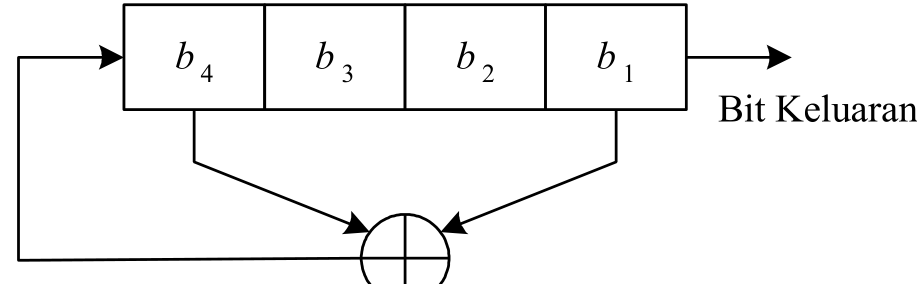
\includegraphics[width=100.38mm,height=78.11mm]{../../images/llm/page_034_img_01.png}%
\end{textblock*}

\end{document}
